%%%%%%%%%%%%%%%%%%%%%%%%%%%%%%%%%%%%%%%%%%%%%%%%%%%%%%%%%%%%%%%%%%%%%%
% This layout was adapted from one found at latextemplates.com which
% was adapted from another.
%
% License: CC BY-NC-SA 3.0
% (http://creativecommons.org/licenses/by-nc-sa/3.0/)
%
% Original header:
%
% This is a LaTeX version of the sample laboratory report from
% Virginia Tech's copyrighted 08-09 CHEM 1045/1046 lab manual.
% Reproduction of this one appendix section for academic purposes
% should fall under fair use.
%
%%%%%%%%%%%%%%%%%%%%%%%%%%%%%%%%%%%%%%%%%%%%%%%%%%%%%%%%%%%%%%%%%%%%%%

\documentclass{article}

\usepackage{graphicx}
%\usepackage[acronym]{glossaries} % Lets us use acronyms
\usepackage{siunitx} % SI units in math mode

\author{}
\title{ELEC-313 \\ Lab 2: Diode Characterization \\ }
\date{\today}

%\loadglsentries{acronyms} % Actually loads 'acronyms.tex'
%\makeglossaries

\begin{document}

\maketitle

\begin{center}
  \begin{tabular}{lr}
    Date Performed: & September 18, 2013 \\
    Partners: & Charles Pittman \\
    & Stephen Wilson \\
  \end{tabular}
\end{center}

\pagebreak

% Removes indentation from paragraphs: \setlength\parindent{0pt}

% Number the enumerate environment (unordered lists) by letter:
\renewcommand{\labelenumi}{\alph{enumi}.}

\section{Objective}
\label{sec:objective}

The objective is to observe the operation of a diode, and its
conformance to the Schlockley equation:
\[I_D = I_S \left(e^{\frac{V_D}{V_T}} - 1\right)\]

\section{Schematics}
\label{sec:schematics}

% The asterisk after section inhibits the numbering of the section.
\subsection*{Circuit Tested}
\label{sec:ckt_tested}

\begin{figure}[hbtp]
  \begin{center}
    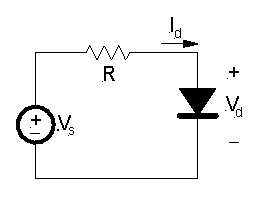
\includegraphics[]{img/circuit1}
  \end{center}
  \caption{\label{fig:circuit1} Circuit used for Part A and Part B.}
\end{figure}

\begin{figure}[hbtp]
  \begin{center}
    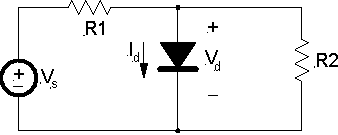
\includegraphics[]{img/circuit2}
  \end{center}
  \caption{\label{fig:circuit2} Circuit used for Part C.}
\end{figure}

\section{Procedure}
\label{sec:procedure}

%First, resistors $R_1$, $R_2$, and $R_3$ were measured with a
%multimeter and recorded in Table~\ref{tab:table_01}.  Then the circuit
%in Figure~\ref{fig:circuit} was constructed on a breadboard.  Next,
%the configuration depicted in Figure~\ref{fig:test_config} was assembled.
%
%Two Fluke multimeters served as the ammeters, and two input channels
%of an oscilloscope served as voltmeters.  The function generator was
%set to produce a sine wave with amplitude of
%\SI{200}{\milli\volt_{rms}} @ \SI{1}{\kilo\hertz}, serving as the
%voltage source, and a decade box set to \SI{200}{\ohm} serving as the
%load.
%
%With the load disconnected, the input voltage ($V_i$), input current
%($I_i$), output voltage ($V_o$), and output current ($I_i$) were
%measured and recorded in Table~\ref{tab:table_02}.  This step was then
%repeated with the load connected.  Using these values with the
%equations derived from the four amplifier models, measured values were
%determined where direct measurement was difficult.

\section{Results}
\label{sec:results}

\subsection{Part A}
\label{sec:result_a}

\begin{figure}[hbtp]
  \begin{center}
    % GNUPLOT: LaTeX picture
\setlength{\unitlength}{0.240900pt}
\ifx\plotpoint\undefined\newsavebox{\plotpoint}\fi
\begin{picture}(1500,900)(0,0)
\sbox{\plotpoint}{\rule[-0.200pt]{0.400pt}{0.400pt}}%
\put(151.0,131.0){\rule[-0.200pt]{4.818pt}{0.400pt}}
\put(131,131){\makebox(0,0)[r]{ 0}}
\put(1419.0,131.0){\rule[-0.200pt]{4.818pt}{0.400pt}}
\put(151.0,196.0){\rule[-0.200pt]{4.818pt}{0.400pt}}
\put(131,196){\makebox(0,0)[r]{ 2}}
\put(1419.0,196.0){\rule[-0.200pt]{4.818pt}{0.400pt}}
\put(151.0,260.0){\rule[-0.200pt]{4.818pt}{0.400pt}}
\put(131,260){\makebox(0,0)[r]{ 4}}
\put(1419.0,260.0){\rule[-0.200pt]{4.818pt}{0.400pt}}
\put(151.0,325.0){\rule[-0.200pt]{4.818pt}{0.400pt}}
\put(131,325){\makebox(0,0)[r]{ 6}}
\put(1419.0,325.0){\rule[-0.200pt]{4.818pt}{0.400pt}}
\put(151.0,389.0){\rule[-0.200pt]{4.818pt}{0.400pt}}
\put(131,389){\makebox(0,0)[r]{ 8}}
\put(1419.0,389.0){\rule[-0.200pt]{4.818pt}{0.400pt}}
\put(151.0,454.0){\rule[-0.200pt]{4.818pt}{0.400pt}}
\put(131,454){\makebox(0,0)[r]{ 10}}
\put(1419.0,454.0){\rule[-0.200pt]{4.818pt}{0.400pt}}
\put(151.0,518.0){\rule[-0.200pt]{4.818pt}{0.400pt}}
\put(131,518){\makebox(0,0)[r]{ 12}}
\put(1419.0,518.0){\rule[-0.200pt]{4.818pt}{0.400pt}}
\put(151.0,583.0){\rule[-0.200pt]{4.818pt}{0.400pt}}
\put(131,583){\makebox(0,0)[r]{ 14}}
\put(1419.0,583.0){\rule[-0.200pt]{4.818pt}{0.400pt}}
\put(151.0,647.0){\rule[-0.200pt]{4.818pt}{0.400pt}}
\put(131,647){\makebox(0,0)[r]{ 16}}
\put(1419.0,647.0){\rule[-0.200pt]{4.818pt}{0.400pt}}
\put(151.0,712.0){\rule[-0.200pt]{4.818pt}{0.400pt}}
\put(131,712){\makebox(0,0)[r]{ 18}}
\put(1419.0,712.0){\rule[-0.200pt]{4.818pt}{0.400pt}}
\put(151.0,776.0){\rule[-0.200pt]{4.818pt}{0.400pt}}
\put(131,776){\makebox(0,0)[r]{ 20}}
\put(1419.0,776.0){\rule[-0.200pt]{4.818pt}{0.400pt}}
\put(151.0,131.0){\rule[-0.200pt]{0.400pt}{4.818pt}}
\put(151,90){\makebox(0,0){ 0}}
\put(151.0,756.0){\rule[-0.200pt]{0.400pt}{4.818pt}}
\put(323.0,131.0){\rule[-0.200pt]{0.400pt}{4.818pt}}
\put(323,90){\makebox(0,0){ 0.1}}
\put(323.0,756.0){\rule[-0.200pt]{0.400pt}{4.818pt}}
\put(494.0,131.0){\rule[-0.200pt]{0.400pt}{4.818pt}}
\put(494,90){\makebox(0,0){ 0.2}}
\put(494.0,756.0){\rule[-0.200pt]{0.400pt}{4.818pt}}
\put(666.0,131.0){\rule[-0.200pt]{0.400pt}{4.818pt}}
\put(666,90){\makebox(0,0){ 0.3}}
\put(666.0,756.0){\rule[-0.200pt]{0.400pt}{4.818pt}}
\put(838.0,131.0){\rule[-0.200pt]{0.400pt}{4.818pt}}
\put(838,90){\makebox(0,0){ 0.4}}
\put(838.0,756.0){\rule[-0.200pt]{0.400pt}{4.818pt}}
\put(1010.0,131.0){\rule[-0.200pt]{0.400pt}{4.818pt}}
\put(1010,90){\makebox(0,0){ 0.5}}
\put(1010.0,756.0){\rule[-0.200pt]{0.400pt}{4.818pt}}
\put(1181.0,131.0){\rule[-0.200pt]{0.400pt}{4.818pt}}
\put(1181,90){\makebox(0,0){ 0.6}}
\put(1181.0,756.0){\rule[-0.200pt]{0.400pt}{4.818pt}}
\put(1353.0,131.0){\rule[-0.200pt]{0.400pt}{4.818pt}}
\put(1353,90){\makebox(0,0){ 0.7}}
\put(1353.0,756.0){\rule[-0.200pt]{0.400pt}{4.818pt}}
\put(151.0,131.0){\rule[-0.200pt]{0.400pt}{155.380pt}}
\put(151.0,131.0){\rule[-0.200pt]{310.279pt}{0.400pt}}
\put(1439.0,131.0){\rule[-0.200pt]{0.400pt}{155.380pt}}
\put(151.0,776.0){\rule[-0.200pt]{310.279pt}{0.400pt}}
\put(30,453){\makebox(0,0){\shortstack{$I_d$\\(mA)}}}
\put(795,29){\makebox(0,0){$V_d$ (V)}}
\put(795,838){\makebox(0,0){Diode Current vs. Voltage}}
\put(627,131){\makebox(0,0){$+$}}
\put(587,131){\makebox(0,0){$+$}}
\put(943,134){\makebox(0,0){$+$}}
\put(1071,146){\makebox(0,0){$+$}}
\put(1130,161){\makebox(0,0){$+$}}
\put(1166,176){\makebox(0,0){$+$}}
\put(1192,192){\makebox(0,0){$+$}}
\put(1212,208){\makebox(0,0){$+$}}
\put(1228,225){\makebox(0,0){$+$}}
\put(1242,241){\makebox(0,0){$+$}}
\put(1254,257){\makebox(0,0){$+$}}
\put(1264,274){\makebox(0,0){$+$}}
\put(1272,291){\makebox(0,0){$+$}}
\put(1281,307){\makebox(0,0){$+$}}
\put(1288,324){\makebox(0,0){$+$}}
\put(1295,341){\makebox(0,0){$+$}}
\put(1302,358){\makebox(0,0){$+$}}
\put(1307,374){\makebox(0,0){$+$}}
\put(1312,392){\makebox(0,0){$+$}}
\put(1317,408){\makebox(0,0){$+$}}
\put(1322,425){\makebox(0,0){$+$}}
\put(1331,459){\makebox(0,0){$+$}}
\put(1339,493){\makebox(0,0){$+$}}
\put(1346,528){\makebox(0,0){$+$}}
\put(1351,562){\makebox(0,0){$+$}}
\put(1358,596){\makebox(0,0){$+$}}
\put(1363,631){\makebox(0,0){$+$}}
\put(1369,665){\makebox(0,0){$+$}}
\put(1374,701){\makebox(0,0){$+$}}
\put(1377,736){\makebox(0,0){$+$}}
\put(1382,771){\makebox(0,0){$+$}}
\put(151.0,131.0){\rule[-0.200pt]{0.400pt}{155.380pt}}
\put(151.0,131.0){\rule[-0.200pt]{310.279pt}{0.400pt}}
\put(1439.0,131.0){\rule[-0.200pt]{0.400pt}{155.380pt}}
\put(151.0,776.0){\rule[-0.200pt]{310.279pt}{0.400pt}}
\end{picture}

  \end{center}
  \caption{\label{fig:part_a_graph} Diode characteristics measured in Part A.}
\end{figure}

\begin{figure}[hbtp]
  \begin{center}
    % GNUPLOT: LaTeX picture
\setlength{\unitlength}{0.240900pt}
\ifx\plotpoint\undefined\newsavebox{\plotpoint}\fi
\sbox{\plotpoint}{\rule[-0.200pt]{0.400pt}{0.400pt}}%
\begin{picture}(1500,900)(0,0)
\sbox{\plotpoint}{\rule[-0.200pt]{0.400pt}{0.400pt}}%
\put(171.0,131.0){\rule[-0.200pt]{4.818pt}{0.400pt}}
\put(151,131){\makebox(0,0)[r]{ 0}}
\put(1419.0,131.0){\rule[-0.200pt]{4.818pt}{0.400pt}}
\put(171.0,239.0){\rule[-0.200pt]{4.818pt}{0.400pt}}
\put(151,239){\makebox(0,0)[r]{ 0.5}}
\put(1419.0,239.0){\rule[-0.200pt]{4.818pt}{0.400pt}}
\put(171.0,346.0){\rule[-0.200pt]{4.818pt}{0.400pt}}
\put(151,346){\makebox(0,0)[r]{ 1}}
\put(1419.0,346.0){\rule[-0.200pt]{4.818pt}{0.400pt}}
\put(171.0,454.0){\rule[-0.200pt]{4.818pt}{0.400pt}}
\put(151,454){\makebox(0,0)[r]{ 1.5}}
\put(1419.0,454.0){\rule[-0.200pt]{4.818pt}{0.400pt}}
\put(171.0,561.0){\rule[-0.200pt]{4.818pt}{0.400pt}}
\put(151,561){\makebox(0,0)[r]{ 2}}
\put(1419.0,561.0){\rule[-0.200pt]{4.818pt}{0.400pt}}
\put(171.0,669.0){\rule[-0.200pt]{4.818pt}{0.400pt}}
\put(151,669){\makebox(0,0)[r]{ 2.5}}
\put(1419.0,669.0){\rule[-0.200pt]{4.818pt}{0.400pt}}
\put(171.0,776.0){\rule[-0.200pt]{4.818pt}{0.400pt}}
\put(151,776){\makebox(0,0)[r]{ 3}}
\put(1419.0,776.0){\rule[-0.200pt]{4.818pt}{0.400pt}}
\put(171.0,131.0){\rule[-0.200pt]{0.400pt}{4.818pt}}
\put(171,90){\makebox(0,0){ 0}}
\put(171.0,756.0){\rule[-0.200pt]{0.400pt}{4.818pt}}
\put(330.0,131.0){\rule[-0.200pt]{0.400pt}{4.818pt}}
\put(330,90){\makebox(0,0){ 0.1}}
\put(330.0,756.0){\rule[-0.200pt]{0.400pt}{4.818pt}}
\put(488.0,131.0){\rule[-0.200pt]{0.400pt}{4.818pt}}
\put(488,90){\makebox(0,0){ 0.2}}
\put(488.0,756.0){\rule[-0.200pt]{0.400pt}{4.818pt}}
\put(647.0,131.0){\rule[-0.200pt]{0.400pt}{4.818pt}}
\put(647,90){\makebox(0,0){ 0.3}}
\put(647.0,756.0){\rule[-0.200pt]{0.400pt}{4.818pt}}
\put(805.0,131.0){\rule[-0.200pt]{0.400pt}{4.818pt}}
\put(805,90){\makebox(0,0){ 0.4}}
\put(805.0,756.0){\rule[-0.200pt]{0.400pt}{4.818pt}}
\put(964.0,131.0){\rule[-0.200pt]{0.400pt}{4.818pt}}
\put(964,90){\makebox(0,0){ 0.5}}
\put(964.0,756.0){\rule[-0.200pt]{0.400pt}{4.818pt}}
\put(1122.0,131.0){\rule[-0.200pt]{0.400pt}{4.818pt}}
\put(1122,90){\makebox(0,0){ 0.6}}
\put(1122.0,756.0){\rule[-0.200pt]{0.400pt}{4.818pt}}
\put(1281.0,131.0){\rule[-0.200pt]{0.400pt}{4.818pt}}
\put(1281,90){\makebox(0,0){ 0.7}}
\put(1281.0,756.0){\rule[-0.200pt]{0.400pt}{4.818pt}}
\put(1439.0,131.0){\rule[-0.200pt]{0.400pt}{4.818pt}}
\put(1439,90){\makebox(0,0){ 0.8}}
\put(1439.0,756.0){\rule[-0.200pt]{0.400pt}{4.818pt}}
\put(171.0,131.0){\rule[-0.200pt]{0.400pt}{155.380pt}}
\put(171.0,131.0){\rule[-0.200pt]{305.461pt}{0.400pt}}
\put(1439.0,131.0){\rule[-0.200pt]{0.400pt}{155.380pt}}
\put(171.0,776.0){\rule[-0.200pt]{305.461pt}{0.400pt}}
\put(30,453){\makebox(0,0){\shortstack{ln($I_d$)\\(mA)}}}
\put(805,29){\makebox(0,0){$V_d$ (V)}}
\put(805,838){\makebox(0,0){Diode Natural Logarithm of Current vs. Voltage}}
\put(1108,203){\makebox(0,0){$+$}}
\put(1132,268){\makebox(0,0){$+$}}
\put(1151,318){\makebox(0,0){$+$}}
\put(1165,360){\makebox(0,0){$+$}}
\put(1177,395){\makebox(0,0){$+$}}
\put(1189,425){\makebox(0,0){$+$}}
\put(1198,451){\makebox(0,0){$+$}}
\put(1206,475){\makebox(0,0){$+$}}
\put(1214,496){\makebox(0,0){$+$}}
\put(1220,516){\makebox(0,0){$+$}}
\put(1227,534){\makebox(0,0){$+$}}
\put(1233,550){\makebox(0,0){$+$}}
\put(1238,566){\makebox(0,0){$+$}}
\put(1242,580){\makebox(0,0){$+$}}
\put(1247,594){\makebox(0,0){$+$}}
\put(1252,606){\makebox(0,0){$+$}}
\put(1260,630){\makebox(0,0){$+$}}
\put(1268,651){\makebox(0,0){$+$}}
\put(1274,671){\makebox(0,0){$+$}}
\put(1279,688){\makebox(0,0){$+$}}
\put(1285,705){\makebox(0,0){$+$}}
\put(1290,720){\makebox(0,0){$+$}}
\put(1295,735){\makebox(0,0){$+$}}
\put(1300,748){\makebox(0,0){$+$}}
\put(1303,761){\makebox(0,0){$+$}}
\put(1307,773){\makebox(0,0){$+$}}
\put(171.0,131.0){\rule[-0.200pt]{0.400pt}{155.380pt}}
\put(171.0,131.0){\rule[-0.200pt]{305.461pt}{0.400pt}}
\put(1439.0,131.0){\rule[-0.200pt]{0.400pt}{155.380pt}}
\put(171.0,776.0){\rule[-0.200pt]{305.461pt}{0.400pt}}
\end{picture}

  \end{center}
  \caption{\label{fig:part_a_graph2} $\ln{(I_d)}$ vs. $V_d$.}
\end{figure}

\subsection{Part B}
\label{sec:result_b}

\begin{table}[hbtp]
  \begin{center}
    \begin{tabular}{ccc}
      $R$ (\si{\ohm}) & $V_d$ (\si{V}) & $I_d$ (\si{mA}) \\
      \hline
      200 & 0.751 & 46.00 \\
      500 & 0.713 & 18.60 \\
      1k & 0.682 & 9.30 \\
      2k & 0.650 & 4.70 \\
      5k & 0.605 & 1.85 \\
      10k & 0.571 & 0.94 \\
      20k & 0.538 & 0.47 \\
      50k & 0.494 & 0.19 \\
      100k & 0.464 & 0.10 \\
    \end{tabular}
  \end{center}
  \caption{\label{tab:part_b} Diode characteristics measured in Part B.}
\end{table}

\begin{table}[hbtp]
  \begin{center}
    \begin{tabular}{ccc}
      $V_d$ (\si{V}) & $I_d$ (\si{mA}) & $V_{OC}$ (\si{V}) \\
      \hline
      0.712 & 27.2 & 6.70 \\
    \end{tabular}
  \end{center}
  \caption{\label{tab:part_b} Diode characteristics measured in Part C.}
\end{table}

\section{Conclusion}
\label{sec:conclusion}

\section{Appendix}
\label{sec:appendix}

\subsection*{Equations}

% LaTeX sees blank lines as a start of another paragraph.  To avoid
% unnecessary vertical spaces between equations, and still visually
% separate in source, put a comment between them.
%\begin{equation}
%  \label{eqn:percent_error}
%  \%_{error} = \frac{|measured - nominal|}{nominal} \times 100\%
%\end{equation}
%%
%\begin{equation}
%  \label{eqn:R_o}
%  R_o = \frac{V_{noload} - V_{load}}{I_{load}}
%\end{equation}
%%
%\begin{equation}
%  \label{eqn:R_i}
%  R_i = \frac{V_i}{I_i}
%\end{equation}
%%
%\begin{equation}
%  \label{eqn:A_v}
%  A_v = \frac{V_o}{V_i}
%\end{equation}
%%
%\begin{equation}
%  \label{eqn:A_i}
%  A_i = A_v \left(\frac{R_i}{R_o}\right)
%\end{equation}
%%
%\begin{equation}
%  \label{eqn:G_m}
%  G_m = \frac{A_v}{R_o}
%\end{equation}
%%
%\begin{equation}
%  \label{eqn:R_m}
%  R_m = A_v R_i
%\end{equation}

\end{document}
